\documentclass[a4paper]{jpconf}
\usepackage{amsmath} % for subequations
\usepackage{xfrac} %to write fractions in different ways
\usepackage{graphicx} %for figures
\usepackage{caption} %for figures
\usepackage{algpseudocode} % to write pseudocode



\begin{document}

\title{The effect of solid objects on the electrostatic potential}
\author{J Cork, T  Hendrick-Beattie, D Lafferty, M Pereira, V Nordgren and N Warrack}
\address{School of Physics and Astronomy, University of Glasgow, Glasgow, UK}

\begin{abstract}
\end{abstract}

\section*{Introduction}
Electromagnetism is one of four fundamental forces of nature. It describes how electrically charged particles interact 
%with each other 
and how they generate electromagnetic fields \cite{Sears.Zamansky-uniPhy}. These fields permeate the space around them, influencing the behaviour of other charges by exerting forces on them. %(that is either attractive or repulsive). 
Electromagnetic forces determine the atomic and macroscopic properties of matter that dominate most of the physical phenomena encountered in daily life such as sound, light and biological processes. Understanding these principles in depth can facilitate significant advances in science and technology. For instance, successful modelling of a simple system of conductors makes it possible to investigate arbitrarily complex configurations of charges which can aid the design of detectors for particle physics. 


%EXTRA
%The electromagnetic force plays a major role in determining the internal properties of most objects encountered in daily life. Ordinary matter takes its form as a result of intermolecular forces between individual molecules in matter. Electrons are bound by electromagnetic wave mechanics into orbitals around atomic nuclei to form atoms, which are the building blocks of molecules. This governs the processes involved in chemistry, which arise from interactions between the electrons of neighboring atoms, which are in turn determined by the interaction between electromagnetic force and the momentum of the electrons.

Electrostatics is the study of stationary or slow-moving electric charges \cite{griffiths-introElec}. They exert electrostatic forces on each other, which in turn are governed by Coulomb's force law and most conveniently described by electric field equations. The relationship between these fields and the distribution of electric charge can be expressed as \cite{griffiths-introElec}

\begin{equation}
\textbf{$\nabla$} \cdot \textbf{E} = \frac{\rho}{\epsilon_0}~,
%\oint \textbf{E} \cdot d\textbf{A} = \frac{Q_{enc}}{\epsilon_0}
\label{eq:intro1}
\end{equation} 

\noindent known as the differential form of Guass's law, where \textbf{$\nabla$} $\cdot$ \textbf{E} is the divergence of the electric field, $\epsilon_0$ is the permittivity of free space and $\rho$ is the charge density. Additionally, for any static charge distribution the electric field is irrotational, \textbf{$\nabla$} $\times$ \textbf{E} $= 0$, therefore the line integral of the electric field
%$\oint \textbf{E} \cdot d \textbf{l} = 0$, 
is independent of the path taken \cite{griffiths-introElec}. This means that \textbf{E} can be written as the gradient of a scalar potential 

\begin{equation}
\textbf{E} = - \nabla V~,
\label{eq:intro2}
\end{equation} 

\noindent where $V$ is called the electric potential, defined as the potential energy per unit charge  \cite{Sears.Zamansky-uniPhy}.
In regions where there is no charge, such that $\rho = 0$, the divergence of the electric field is zero. Hence, using Eq.(\ref{eq:intro1}) and Eq.(\ref{eq:intro2}) the electric potential
%for any point in space 
can be described by

\begin{equation}
\nabla^2 V = 0~.
\label{eq:intro3}
\end{equation} 

\noindent This is Laplace's equation \cite{RHB-MathematicalMethods}.\\ \par
In this work, the electrostatic potential and the electric field are evaluated at all points in two different systems. The systems consist of different geometric configurations of conductors held at constant potentials. This study shows how the $V$ is modified in the presence of these conductors. 

\section*{Methods}
In general, there are two methods to analyse the electric potential in all space: analytical and numerical techniques. Often there is no analytical solution, even for a simple electrostatic system, and thus numerical methods are useful tools in obtaining approximate solutions. 

\subsection*{Analytical Approach} 
%Partial differential equations (PDE) are fundamental to describe physical phenomena, such as heat, fluids, electrostatics, sound and so on. This is an equation that involves an unknown function of two or more variables and their partial derivatives. A particular solution may be specified from the general solution of a PDE in the presence of boundary conditions. \par
%The electric field is dominated by inherent symmetries that are better described in  coordinates \cite{RHB-MathematicalMethods} in which

For systems with certain symmetries Laplace's equation can be expressed in cylindrical coordinates \cite{RHB-MathematicalMethods}, namely
 
\begin{equation}
\frac{1}{s}\frac{\partial}{\partial s}\bigg(s \frac{\partial V}{\partial s}\bigg) + \frac{1}{s^2} \frac{\partial^2 V}{\partial \phi^2} + \frac{\partial^2 V}{\partial z^2} = 0~.
\label{eq:1}
\end{equation}

%For round objects $\Phi$ can be independent of $\phi$ given an appropriate choice of coordinate orientation. Multiplying through by $r^2$ the equation is simplified to

\noindent For an axisymmetrical system the electrostatic potential will not depend on $z$. This implies that $\sfrac{\partial^2 V}{\partial z^2} = 0~.$ Multiplying through by $s^2$ the equation is simplified to

\begin{equation}
s \frac{\partial}{\partial s}\bigg(s \frac{\partial V}{\partial s}\bigg) + \frac{\partial^2 V}{\partial \phi^2} = 0~.
\label{eq:2}
\end{equation}

Separation of variables is used to solve the equation above. Let $V(s,\phi) = S(s)\Phi(\phi)$, where the factors $S$ and $\Phi$ are functions of $s$ and $\phi$ respectively. Substituting for and dividing through by $V$, Eq.(\ref{eq:2}) can be written as 

\begin{equation}
\frac{s}{S}\frac{d}{ds}\bigg(s \frac{dS}{ds}\bigg) + \frac{1}{\Phi}\frac{d^2 \Phi}{d \phi^2} = 0~.
\label{eq:3}
\end{equation}

\noindent This form shows that the first term depends only on $s$, and the second only on $\phi$. It follows that  each term is equal to a constant defined, for convenience, to be $k^2$:

\begin{subequations}
\begin{align}
&s\frac{d}{ds}\bigg(s \frac{dS}{ds}\bigg) = k^2 S, \label{eq:4.1}\\ 
&\frac{d^2 \Phi}{d \phi^2} = - k^2 \Phi ~. \label{eq:4.2}
\end{align}
\label{eq:4}
\end{subequations} 

\noindent The partial differential equation, Eq.(\ref{eq:2}), has been converted into two independent ordinary differential equations. The general solution for the angular part, Eq.(\ref{eq:4.2}), is

\begin{equation}
\Phi(\phi) = A_k cos(k \phi) + B_k sin(k \phi)~,
\label{eq:phi}
\end{equation}

\noindent where $A_k$ and $B_k$ are arbitrary constants \cite{RHB-MathematicalMethods}. The condition $\Phi(\phi) = \Phi(\phi + 2 \pi)$ is required so that the potential is single valued, this implies that $k$ must be an integer. %APPENDIX??
When $k = 0$ Eq.(\ref{eq:4.2}) has solution $\Phi(\phi) = B_0 \phi + A_0$, where $B_0 = 0$ in order to satisfy this condition and $A_0$ is an arbitrary constant. \\ \\ \par 
Eq.(\ref{eq:4.1}) has solutions $s^k$ and $s^{-k}$ by inspection \cite{griffiths-introElec}. The general solution has the form

\begin{equation}
S(s) = C_k s^k + D_k s^{-k}
\label{eq:s}
\end{equation} 

\noindent where $C_k$ and $D_k$ are arbitrary constants. For $k = 0$, Eq.(\ref{eq:4.1}) takes the form

\begin{equation}
S(s) = C_0 \ln{s} + D_0~,
\label{eq:s2}
\end{equation}

\noindent where $C_0$ and $D_0$ are, again, arbitrary constants. This formula is known as the potential of an infinitely long line or cylinder of uniform charge density. \par
%Furthermore, when $k = 0$ Eq.(\ref{eq:4.2}) has solution $\Phi(\phi) = B_0 \phi + A_0$, where $B_0$ and $A_0$ are arbitrary constants. However, the term $B_0 \phi$ is unacceptable because it does not return to its initial value when $\phi$ is increased by $2 \pi$. \par

%However, the general solution for the angular equation, Eq.(\ref{eq:4.2}), requires Legendre Polynomials in the variable $\cos \theta$. These are special functions usually encountered in physical problems involving Laplace's equation \cite{RHB-MathematicalMethods}. The solution has the form
%\begin{equation}
%\Theta(\theta) = P_{s}(\cos \theta)~,
%\label{eq:5}
%\end{equation} where $P_s$ is the $s$th-order polynomial in $x$ and can be expressed using the Rodrigues' formula \cite{RHB-MathematicalMethods}
%\begin{equation}
%P_s(x) = \frac{1}{2^s s!} \frac{d^s}{dx^s}(x^2 -1)^s~.
%\label{eq:6}
%\end{equation}

%\noindent Therefore, the most general separable solution is:
%\begin{equation}
%\Phi(r, \theta) = \bigg(A r^s + \frac{B}{r^{s+1}}\bigg) P_s (\cos \theta)~.
%\label{eq:7}
%\end{equation}  

Since Laplace's equation is a linear PDE, the general solution is a superposition of all solutions corresponding to different allowed values of $k$ \cite{griffiths-introElec}. The linear combination can be written as
%\begin{equation}
%\Phi(r, \theta) = \sum_{s=0}^{\infty} \bigg( A_s r^s + \frac{B_s}{r^{s+1}}\bigg) P_s (\cos \theta)~,
%\label{eq:8}
%\end{equation} where $A_s$ and $B_s$ are arbitrary constants that are determined by boundary conditions. 

\begin{equation}
V(s, \phi) = A_0 (C_0 \ln{s} + D_0) + \sum_{k=1}^{\infty} \big[(A_k \cos{(k\phi)} + B_k \sin{(k\phi)}) (C_k s^k + D_k s^{-k})\big]
\label{eq:gs1}
\end{equation}
\noindent and simplified to
\begin{equation}
V(s, \phi) = c_0 \ln{s} + d_0 + \sum_{k=1}^{\infty} \big[ s^k (a_k \cos{(k\phi)} + b_k \sin{(k\phi)}) + s^{-k}(c_k \cos{(k\phi)} + d_k \sin{(k\phi)})\big]
\label{eq:gs2}
\end{equation}
\noindent where $c_0, d_0, a_k, b_k, c_k$ and $d_k$ are arbitrary constants that will be determined by boundary conditions. 
\\ \par 

\subsection*{Numerical Techniques}
%\cite{Press.T.V.F-NumericalRecipes}
%Laplace?s equation is mathematically described as an elliptic PDE due to its characteristics. To find a particular solution for this differential equation additional conditions must be imposed. These conditions are boundary values that describe all or part of the perimeter of the region in which a solution is desired. The nature of these boundary conditions usually determines the numerical method required to obtain an approximate solution [4]. This is called a Boundary value problem, specifically an Elliptic boundary value problem which does not involve a time variable.

To find a particular solution for a differential equation, boundary conditions must be imposed that describe all or part of the region in which the solution is desired. The nature of these boundary conditions determines the numerical method required to obtain an approximate solution \cite{Cheney.Kincai-NumericalMethods}. \par
Laplace's equation is an elliptic PDE due to its mathematical characteristics and these are fundamental to its physical significance \cite{RHB-MathematicalMethods}. Problems that are governed by elliptic PDEs and subjected to boundary conditions are called Boundary value problems.
These problems can be solved by Finite-difference and Relaxation methods. \par

The first step of the numerical technique is to discretize the problem by defining a mesh; a grid of  spatial points that cover the domain of interest. The points that lie on the mesh can be written in cartesian coordinates as 

\begin{subequations}
\begin{align}
&x_i = ih\\ 
&y_j = jh
\end{align}
\label{eq:coord}
\end{subequations} 

\noindent where $h$ is the distance between the grid points and $i,j$ is a pair of indices describing each grid point. The differential operator $\nabla^2$ is then approximated 
to a discrete form through the use of finite differences. The standard approximation for the second derivative is \cite{Cheney.Kincai-NumericalMethods} 

\begin{equation}
f''(x) \approx \frac{1}{h^2}[f(x+h) - 2f(x) + f(x-h)].
\end{equation}

\noindent Since there are two variables, $x$ and $y$, the discrete approximation to the the Laplacian can be written as

\begin{equation}
\nabla^2 V \approx \frac{V(x+h,y) + V(x-h,y) - 2V(x,y)}{h^2} + \frac{V(x,y+h) + V(x,y-h) - 2V(x,y)}{h^2}~,
\end{equation}

\noindent or in grid notation,

\begin{equation}
(\nabla^2 V)_{ij} \approx \frac{1}{h^2}[V_{i+1,j} + V_{i-1,j} + V_{i,j+1} + V_{i,j-1} - 4V_{i,j}]~.
\label{eq:fivepoint}
\end{equation}

\noindent This equation is called the Five-point formula \cite{Cheney.Kincai-NumericalMethods}. The name comes from the fact that the value of $V$ at some point $(x,y)$ is related to the four nearest grid points. Substituting $(\nabla^2 V)_{ij}$ = 0 into Eq.(\ref{eq:fivepoint}) gives 

\begin{equation}
V_{i,j} = \frac{1}{4}(V_{i+1,j} + V_{i-1,j} + V_{i,j+1} + V_{i,j-1})~,
\end{equation}

\noindent which shows that a solution to Laplace's equation has the property that at any point it is equal to the average of the values at neighbouring points. The inherent truncation error in the Five-point formula is of order $\mathcal{O}(h^2)$ \cite{Cheney.Kincai-NumericalMethods}.  \par

An alternative method is the Nine-point formula where the eight nearest neighbours are used: horizontal, vertical and diagonal. It can be written as

%\begin{equation}
%(\nabla^2 V)_{ij} \approx \frac{1}{6h^2}[4V_{i+1,j} + 4V_{i-1,j} + 4V_{i,j+1} + 4V_{i,j-1} + V_{i+1,j+1} V_{i-1,j+1} + V_{i+1,j-1} + V_{i-1,j-1} - 20V_{i,j}]~.
%\end{equation}
%\noindent which can be simplified to

\begin{equation}
V_{i,j} = \frac{1}{20}(4V_{i+1,j} + 4V_{i-1,j} + 4V_{i,j+1} + 4V_{i,j-1} + V_{i+1,j+1} V_{i-1,j+1} + V_{i+1,j-1} + V_{i-1,j-1})~.
\end{equation}

\noindent This formula provides an approximation with an error of $\mathcal{O}(h^4)$ when applied to Laplace's equation \cite{AI-numericalAna}. 

The boundary conditions are then specified in the mesh and the interior points of the region desired are assigned to arbitrary values. The chosen values will not influence the final solution but they may affect the rate of convergence of the scheme. \par

The iterative method to solve Laplace's equation re-evaluates each $V_{i,j}$ to the average of the four or eight nearest points. The process is repeated until the change between successive iterations is too small according to a specified error tolerance, and an approximate solution is obtained. 
%The iterative method to solve Laplace's equation starts by guessing a solution and then sweeps across the grid updating the value at each point. On each interation $V_{i,j}$ is set to the average of the four or eight nearest points. 
%Initially the result will not be exact since the neighbours also get updated, but by repeating the process several times the scheme converges to a solution. When the change between iterations is two small, according to a specified error tolerance, a solution is obtained. 
This procedure is a relaxation technique called the Jacobi method. This method is generally slow but Gauss-Seidel method can be implemented in order to improve it. \par

Gauss-Seidel method generally has a faster convergence and requires less memory \cite{Cheney.Kincai-NumericalMethods}. It uses the updated values immediately to compute the next ones. In this way most points will be calculated using the values from previous and current iterations at the same time. For the Five-point formula this can be expressed as

\begin{equation}
V_{i,j}^{n+1} = \frac{1}{4}(V_{i+1,j}^{n} + V_{i-1,j}^{n+1} + V_{i,j+1}^{n} + V_{i,j-1}^{n+1})~.
\end{equation}

\noindent where $n$ is the iteration number. 

The accuracy of the numerical approximation improves as the number of points in the mesh increases for both numerical formulas, Five-point and Nine-point. This can be done by implementing Adaptive meshing \cite{Press.T.V.F-NumericalRecipes}. The Relaxation method is applied to an uniform mesh and then the solution is examined to determine where more grid points should be added. A finer subgrid is superimposed in the regions requiring more resolution. The procedure is then repeated with the improved mesh until the local error has dropped below a desired level. This refinement decreases the uncertainty in the numerical solution.


\section*{Solving a physical system}
There are simple electrostatic systems for which an analytical solution can be derived. These systems can be extremely helpful when developing a numerical solution. They are used to ensure the correctness and the accuracy of the numerical approximation. In this work, a system consisting of two infinitely long plates and a conducting cylinder was used to serve this purpose. Due to symmetry this 3D system can be approximated to a 2D 


 %A long conducting cylinder is placed into the field at ground potential between the plates. 

\begin{figure}[h]
	\centering
	\includegraphics[width=6cm]{GPdiagram11} 
	\caption{Illustration of system $A$. A perfectly uniform field is defined between plates $+V$ and $-V$. An uncharged conducting cylinder of radius $R$ is placed in the middle of the system (cross-section view).}
	\label{fig:systemA}
\end{figure}


When an uncharged cylindrical conductor is placed between two parallel charged plates, the electric field is altered. The field pushes free positive charges to the right and the negative ones to the left. The charges accumulate in the edges of the conductor distorting the field in the surroundings of the cylinder. The potential outside the conductor can be described mathematically using principles of electrostatics, namely Laplace's Equation Eq.(\ref{eq:intro3}). %This PDE describes the electrostatic potential for a given charge distribution, and consequently the corresponding field. 
A particular solution defining System $A$ is obtained using Eq.(\ref{eq:gs2}) and the required boundary conditions. \\ \\ 


The potential at the surface of a grounded conductor is zero \cite{griffiths-introElec}. Also, far from the cylinder the field is perpendicular to the plates, so at infinity $\bf{E}$ = $E_0$$\bf{\hat{x}}$, hence $V = -E_0 x + C$, where C is an arbitrary constant and $E_0$ is the initial electric field. Due to the symmetry of the system, $V$ is known to be zero at the same distance from the plates. In cylindrical coordinates, this becomes $V(s,\phi) = -E_0 s \cos{\phi}$. Therefore, the boundary conditions can be expressed as

\begin{subequations}
\begin{align}
&V = 0  \hspace{75pt} s = R~,\\ 
&V \to -E_0 s \cos{\phi} \hspace{27pt} s \gg R~,
\end{align}
\end{subequations}

\noindent where $R$ is the radius of the sphere as shown in Fig.\ref{fig:systemA}. In order to have the right boundaries at infinity $C_0 = D_0 = b_k = d_k=0$, and $a_k = b_k=0$ except for $k=1$. Therefore,

\begin{equation}
V(s,\phi) = \bigg( a_1 s + \frac{c_1}{s}\bigg) \cos{\phi}~.
\label{eq:V1}
\end{equation}

The first boundary condition implies that Eq.(\ref{eq:V1}) is zero, hence

\begin{equation}
\bigg( a_1 R + \frac{c_1}{R}\bigg) \cos{\phi} = 0~,
\end{equation} 

\noindent or 

\begin{equation}
c_1 = - a_1 R^2 ~.
\end{equation}

\noindent The second condition requires Eq.(\ref{eq:V1}) to be equal to $-E_0 s \cos{\phi}$. By rearranging the expression and substituting in $c_1$ this takes the form

\begin{equation}
a_1 s = -E_0 s + \frac{a_1 R^2}{s}~.
\end{equation}

\noindent For $s \gg R$ the term $(\sfrac{a_1 R^2}{s})$ goes to zero, so $a_1 = -E_0$.
%$P_s(\cos \theta)$ is not always zero, therefore
%\begin{equation}
%A_s R^s + \frac{B_s}{R^{s+1}} = 0~,
%\end{equation}
%or
%\begin{equation}
%B_s = -A_s R^{2s+1}~.
%\end{equation}
Using Eq.(\ref{eq:V1}), $a_1$ and $c_1$ the potential $V(s,\phi)$ can be written as

\begin{equation}
V(s,\phi) = - E_0 \bigg(s - \frac{R^2}{s}\bigg) \cos{\phi}~.
\label{eq:V2}
\end{equation}

%\begin{equation}
%\Phi(r,\theta) = \sum_{s=0}^{\infty} A_s \bigg(r^s - \frac{R^{2s+1}}{r^{s+1}}\bigg) P_s (\cos \theta)~.
%\end{equation}
%
%\noindent For $r\gg R$ the term $(\sfrac{R^{2s+1}}{r^{s+1}})$ goes to zero, therefore the second condition requires that
%
%\begin{equation}
%\Phi(r,\theta)=\sum_{s=0}^{\infty} A_s r^s P_s(\cos \theta) = -E_0 r \cos \theta~,
%\label{eq:14}
%\end{equation}
%
%\noindent since there is only one term in this summation, $s=1$. So $P_s(\cos \theta)= \cos \theta$ and $A_1 = -E_0$ and $A_{s \ne 1} = 0$. Therefore, Eq.(\ref{eq:14}) becomes
%
%\begin{equation}
%\Phi(r,\theta) = -E_0 \bigg(r - \frac{R^3}{r^2}\bigg) \cos \theta~.
%\end{equation}

\noindent The particular solution describing system A is then

\begin{equation}
V(s,\phi) = \left\{ 
  \begin{array}{l l}
   -E_0 \big(s - \frac{R^2}{s}\big) \cos{\phi}  & \qquad \text{for $s > R$}\\
    0 & \qquad \text{for $s \le R$}
  \end{array} \right.
\end{equation}

\noindent or in cartesian coordinates, 

\begin{equation}
V(x,y) = \left\{ 
  \begin{array}{l l}
   -E_0 x \big(1 - \frac{R^2}{x^2 + y^2}\big) & \qquad \text{for $\sqrt{x^2 + y^2} > R$}\\
    0 & \qquad \text{for $\sqrt{x^2 + y^2} \le R$~.}
  \end{array} \right.
  \label{eq:cartesian}
\end{equation}

%In order to compare numerical and analytical solutions the latter had to be implemented in a computer program. The boundaries were specified to 1V and -1V at the plates and 0V inside the cylinder. The electric field $E_0$ was defined as ratio of the voltage difference between the plates and the plate separation. Then using Eq.(\ref{eq:cartesian}) the potential was calculated at all points on a discretized grid. \\
%

Values of the analytical solution of system A were calculated using Eq.(\ref{eq:cartesian}) for discrete values of $x$ and $y$ to allow for comparison with the numerical. The initial electric field, $E_0$, was defined as

\begin{equation}
	E_0 = \frac{\Delta V}{d},
\end{equation} 

\noindent where $d$ is the plate separation and $\Delta V$ is the potential difference between the plates. The potentials at the plates were defined as +1V and -1V. \\

%
%The Finite-difference and Relaxation methods described were utilised in a C++ program to solve system $A$ numerically.
%The plates and the grounded cylinder were defined in a matrix to hold the required values, just as in the analytical case. They remained constant throughout the program and the rest of the elements in the matrix were allowed to vary. The numerical algorithm described, Nine-point formula, was run updating the elements in the matrix until the change in all values between two iterations was considered sufficiently small. This small change was determined using the requested error tolerance. Upon each iteration, the previous iterations values were stored in a temporary array.  When the system was considered stable, the elements in the matrix were further granulated depending on the steepness of their gradients.
%When the scheme finished, the resulting matrix was then plotted using a plotting package where a heat-map functionality was used to depict the potential. For the fieldlines, a further calculation was required: the gradient between each pixel is calculated and used to plot the electric field. The program flow can be seen in Fig.\ref{fig:prog}. 

The Gauss-Seidel method described was implemented in C++. Initial values pertaining to system A were imposed, and with a starting matrix containing only the boundary values, the algorithm was run until no point on the matrix changed by more than a user-defined percentage between two iterations. A method of adaptive meshing was then applied, the level of granulation depending on the gradient of the potential and the maximum granulation being user-defined. This meshed system was refined further by applying the Gauss-Seidel method again for several more iterations, and finally plotted as a heatmap showing potential. (See Fig.(\ref{fig:prog}) for a more detailed programme flow.)

%ALGORITHM (not completed)
%\subsection*{Pseudocode}
%\begin{algorithmic}
%
%\State{matrix $M_{m \times n \times 2}$}
%\State{integer $m =$ row size}
%\State{integer $n =$ column size}
%\State{integer $count =$ 0}
%\While{gradient condition not met}
%	\For{row from 0 to $m$}
%		\For{column from 0 to $n$}
%			\State{$i = count$ mod 2}
%			\State{$j = ( count + 1 )$ mod 2}
%			\If{point is to remain constant (e.g. positive plate)}
%				\State{$M_{row,column,j} = M_{row,column,i}$}
%			\Else
%				\State{$left = M_{row,column-1,i}$}
%				\State{$right = M_{row,column+1,i}$}
%				\State{$above = M_{row-1,column,i}$}
%				\State{$below = M_{row+1,column,i}$}
%				
%				\If{point in top-left}
%					\State{$M_{row,column,j} = 0.5 \times ( right + below )$}
%				\ElsIf{point in top-right}
%					\State{$M_{row,column,j} = 0.5 \times ( left + below )$}
%				\ElsIf{point in bottom-left}
%					\State{$M_{row,column,j} = 0.5 \times ( right + above )$}
%				\ElsIf{point in bottom-right}
%					\State{$M_{row,column,j} = 0.5 \times ( left + above )$}
%				\ElsIf{point in top row}
%					\State{$M_{row,column,j} = \sfrac{1}{3} \times ( right + left + below )$}
%				\ElsIf{point in bottom row}
%					\State{$M_{row,column,j} = \sfrac{1}{3} \times ( right + left + above )$}
%				\ElsIf{point in leftmost column}
%					\State{$M_{row,column,j} = \sfrac{1}{3} \times ( right + above + below )$}
%				\ElsIf{point in rightmost column}
%					\State{$M_{row,column,j} = \sfrac{1}{3} \times ( right + above + below )$}
%				\Else
%					\State{$M_{row,column,j} = \sfrac{1}{4} \times ( right + above + below )$}
%				\EndIf
%			
%				
%			\EndIf
%		\EndFor
%	\EndFor
%\EndWhile
%\end{algorithmic}

\begin{figure}[h]
	\centering
	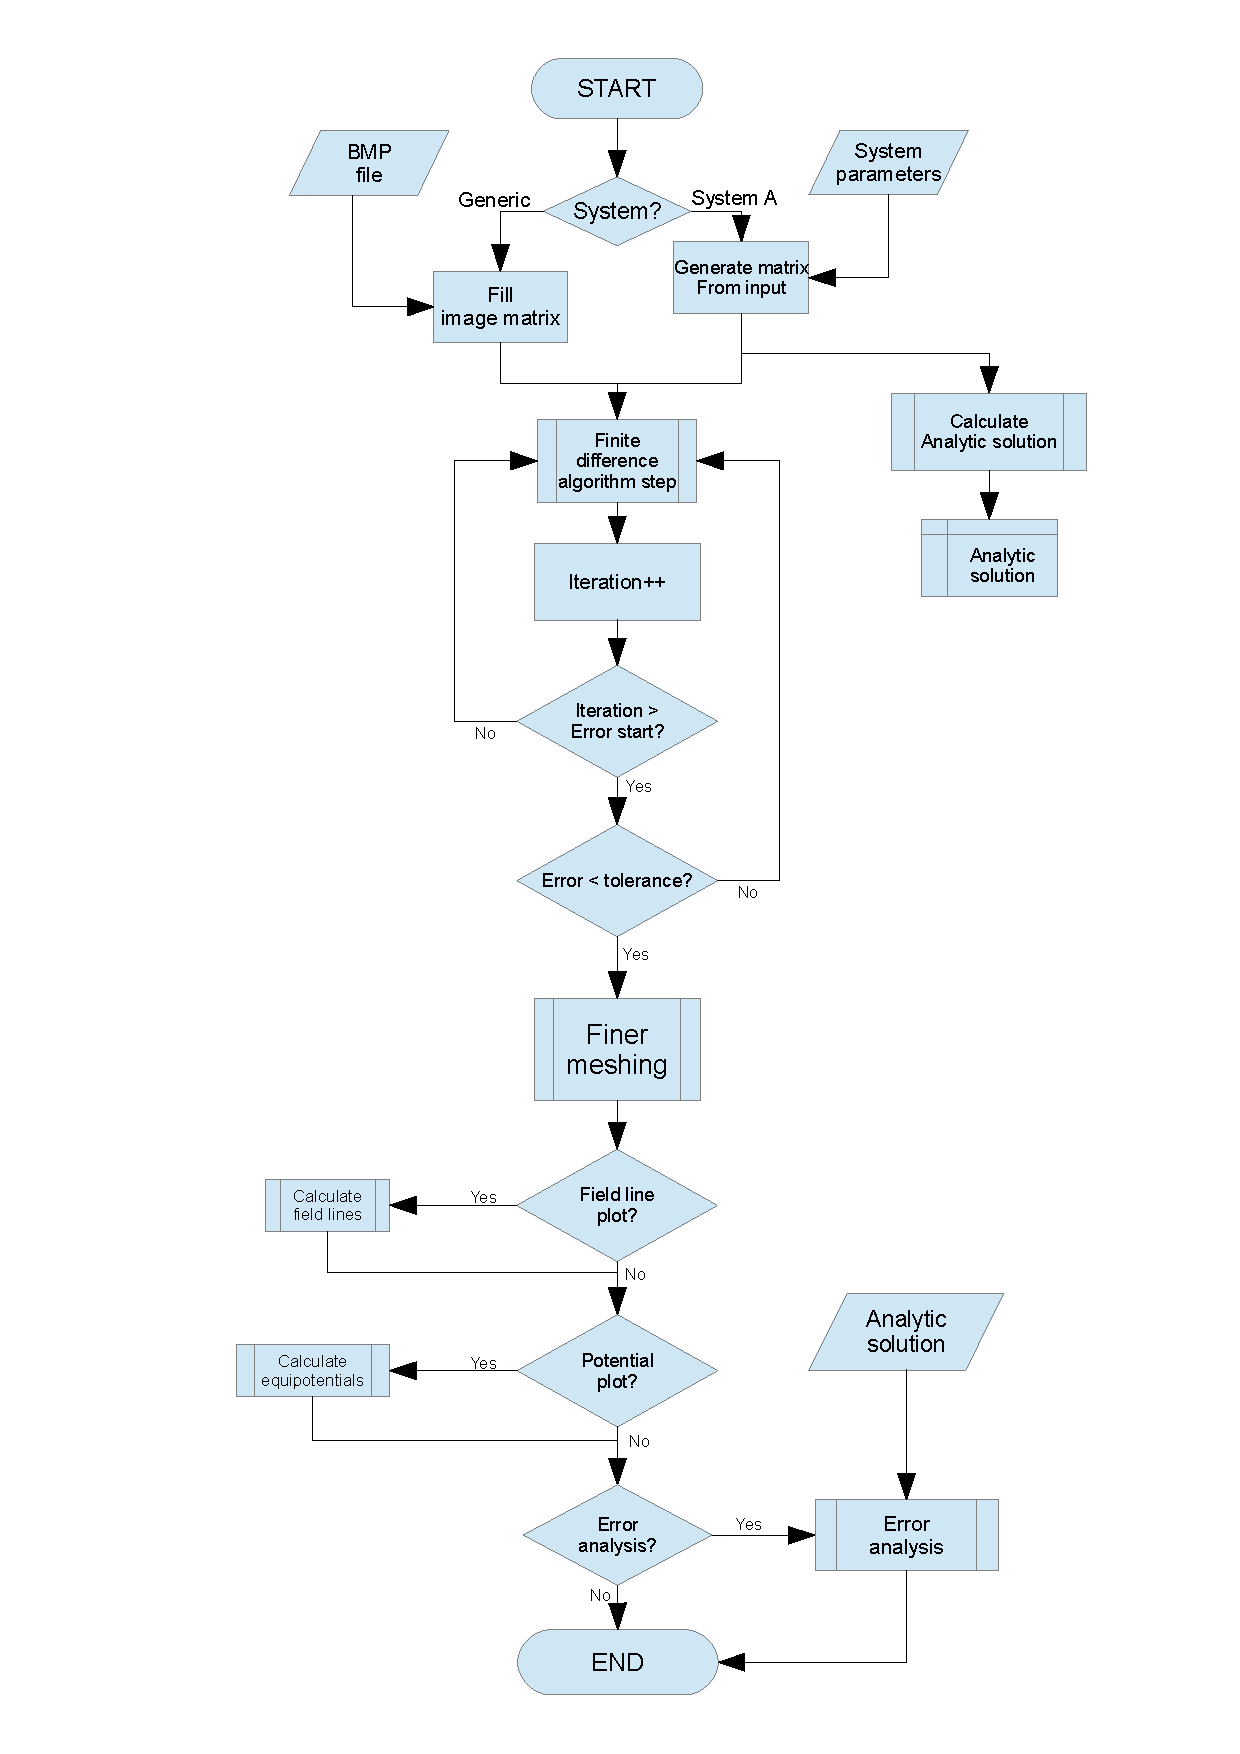
\includegraphics[width=13cm]{progflow} 
	\caption{Program Flow}
	\label{fig:prog}
\end{figure}

\section*{Results and Discussion}

\section*{System E}
% BITMAP %TALK WITH NEIL
%A pixelated drawing describing the components of the system, a bitmap, was passed to the program. Each pixel was then mapped to a matrix holding values between -1 and 1, to represent the voltages of the initial system. The matrix elements related to components, that is, conductors or charges, were not changed during the numerical procedure while the rest varied as the program run.


\begin{figure}[h]
	\centering
	\includegraphics[width=8cm]{GPdiagram21} 
	\caption{systemB}
	\label{fig:systemB}
\end{figure}

\section*{Conclusion}

\section*{References}
\bibliographystyle{ieeetr}
\bibliography{Bibliography3rdYear}

\end{document}
